\documentclass{article}
\usepackage{ctex}
\usepackage{amsmath}
\usepackage{amsthm}
\usepackage{amssymb}
\usepackage{graphicx}
\usepackage{tikz}
\newtheorem{theorem}{定理}
\title{ass01 集合的包含关系使集合是偏序的}
\date{}
\author{}
\begin{document}
\maketitle

\section{定理翻译及证明}

\begin{theorem}
    设\(A\)、\(B\)、\(C\)是集合,如果\(A \subseteq B\)且\(B \subseteq C\),那么\(A \subseteq C \)。
    如果 \(A \subseteq B\) 并且 \(B \subseteq A\),那么 \(A = B\)。
    最后,如果 \(A \subsetneq B\) 并且 \(B \subsetneq C\),那么 \(A \subsetneq C\)。\cite[p.32]{Tao2016AnalysisI}
\end{theorem}

\begin{figure}[h] 
    \centering 
    \includegraphics[width=0.5\textwidth]{setinclusion.png}
    \caption{集合的包含关系示意图}
    \label{fig:example1}
\end{figure}

\begin{figure}[h]
    \centering
    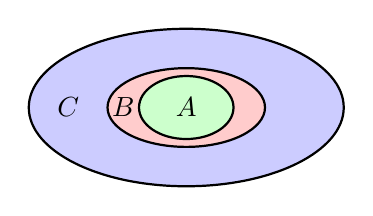
\begin{tikzpicture}
        % C
        \draw[thick,fill=blue!20](0,0)ellipse(2cm and 1cm);
        \node at (-1.5,0){$C$};

        % B
        \draw[thick,fill=red!20](0,0)ellipse(1cm and 0.5cm);
        \node at (-0.8,0){$B$};

        % A
        \draw[thick,fill=green!20](0,0)ellipse(0.6cm and 0.4cm);
        \node at (0,0){$A$};
    \end{tikzpicture}
    \caption{集合的包含关系示意图}
    \label{fig:example2}
\end{figure}

\begin{proof}
    我们只证明第一个结论。假设\(A \subseteq B\)且\(B \subseteq C\),为了证明\( A \subseteq C\),我们必须证明\(A\)中的每一个元素都是\(C\)中的元素。
    那么取\(A\)中的任意一个元素\(x\),因为\(A \subseteq B\),所以\(x\)一定是\(B\)中的元素。又因为\(B \subseteq C\),所以\(x\)是
    \(C\)中的元素。因此\(A\)中的每一个元素实际上都是\(C\)中的元素,结论得证。
\end{proof}

\section{选择理由}
    这一定理指出集合的包含关系是一个偏序关系,是集合论的基础定理之一。集合论在后续课程的学习中经常会用到,如概率论
    第一章就有所涉及。任取集合中的一个元素证明集合的相关性质也是常用手段,如数学分析三中对开集、闭集性质的一些证明就用到这一方法。

\bibliography{ass01.bib}
\bibliographystyle{plain}

\end{document}